\documentclass[a4paper,12pt]{article}
\usepackage[top=2cm, bottom=2cm, left=2.5cm, right=2.5cm]{geometry}
\usepackage[utf8]{inputenc}
\usepackage{amsmath, amsfonts, amssymb}
\usepackage{graphicx}
\usepackage{float}
\usepackage[brazil]{babel}
\usepackage{indentfirst}
\DeclareMathOperator{\sen}{sen}
\DeclareMathOperator{\tg}{tg}
\DeclareMathOperator{\cossec}{cossec}
\newcommand{\limite}{\displaystyle\lim}
\newcommand{\integral}{\displaystyle\int}
\newcommand{\soma}{\displaystyle\sum}
\title{Aqui vem o título do trabalho}
\author{Geovanni Fernandes Garcia \\ geovanni@usp.br}


\begin{document}
\maketitle
\tableofcontents
\listoffigures
\listoftables \newpage

\section{Formatação}

\subsection{Posição do Texto}

\begin{center}
\textbf{Equação polinomial do 2º grau}
\end{center}

Uma equação da forma $$ax^2 + bx + c = 0,$$ com $a \neq 0$ será chamada de
equação polinomial do 2º grau.

A solução dessa equação é dada por:
$$x = \frac{-b \pm \sqrt{b^2 - 4ac}}{2a}$$

\subsection{Itens enumerados}

\begin{enumerate}
 \item aaaaaaaaaa
  \begin{enumerate}
   \item esse é um texto
    \begin{enumerate}
     \item item i eu acho
     \item deve ser o ii
    \end{enumerate}
   \item esse é outro texto
   \item esse mais outro
  \end{enumerate}
 \item bbbbbbb
\end{enumerate}

\begin{itemize}
 \item aaaaa
  \begin{itemize}
   \item não sei
   \item não sei também
  \end{itemize}
 \item bbbb
 \item cccccc
\end{itemize}

\subsection{Expressões Matemáticas}

$a + b$

$a - b$

$a\cdot b$

$a\times b$

$a\div b$

$\frac{a}{b}$, $\dfrac{a}{b}$

$\sqrt[b]{a}$

$a^{b+c}$

$a_1$, $a_2$, $a_3$, ... $a_{n-1}$, $a_n$

\subsection{Notação de Conjuntos}

\begin{enumerate}
 \item Sejam os conjuntos $A = \{1,2,3,4\}$, $A = \{1,\,2,\,3,\,4\}$,
 $B = \{x \in \mathbb{Z} \,|\, -2 \leq x < 4 \}$ e
 $C = \{x \in \mathbb{N} \,|\, x \geq 2 2\}$. Responda aos itens abaixo:
 \begin{enumerate}
  \item $A \cap B$
  \item $B \cup C$
  \item $A - C$
  \item $C \setminus B$
 \end{enumerate}
 \item Classifique em verdadeiro ou falso:
 \begin{enumerate}
  \item $\mathbb{Z} \not\subset \mathbb{N}$.
  \item $\mathbb{R} \not\supset \mathbb{Q}$.
  \item $0 \not\in \mathbb{R}\setminus\mathbb{Q}$.
  \item $\forall x \in \mathbb{N}$, temos
  $x \geq 0$.
  \item $\exists x \in \mathbb{R}$, tal que
  $\sqrt{x}\not\in\mathbb{R}$.
  \item $7 \not\in \{x\in\mathbb{N} \,|\,
  x\textrm{ é par}\}$
  \item $-5 \in \mathbb{R}^*_+$
  \item $0 \in \varnothing$
 \end{enumerate}
 
\subsection{Notação de Função} 
 
 \item Seja a função $f : \mathbb{R}^*_+ \to \mathbb{R}$
 definida por:
 $$f(x) =
  \begin{cases}
   x^2 - 1\,,\textrm{ se }\,x \geq 1 \\
   x - 3 \,,\textrm{ se }\,-1 \leq x < 1 \\
   2x + 1 \,,\textrm{ se }\,x < -1
  \end{cases}
 $$
 \begin{enumerate}
  \item Esboce o gráfico da função.
  \item Calcule o $\log_2 x$ e o $\ln x$.
  \item Encontre os valores de $\cos x$,
  $\sen \left(x - \dfrac{\pi}{2}\right)$,
  $\tg \left(e^x - e^{-x}\right)$ e
  $\cossec \left(\sqrt{\dfrac{a^2 - b^2}{a^2 + b^2}}\right)$.
 \end{enumerate}
 
\subsection{Notação de Matriz} 
 
 \item Considere o produto matricial $A \cdot X = B$ a seguir: 
  $$
  \begin{pmatrix}
   a_{11} & a_{12} & a_{13} & \cdots & a_{1n} \\
   a_{21} & a_{22} & a_{23} & \cdots & a_{2n} \\
   a_{31} & a_{32} & a_{33} & \cdots & a_{3n} \\
   \vdots & \vdots & \vdots & \ddots & \vdots \\
   a_{m1} & a_{m2} & a_{m3} & \cdots & a_{mn}
  \end{pmatrix}
  \begin{pmatrix}
   x_1 \\ x_2 \\ x_3 \\ \vdots \\ x_n
  \end{pmatrix}
  =
  \begin{pmatrix}
   b_1 \\ b_2 \\ b_3 \\ \vdots \\ b_n
  \end{pmatrix}
  $$
  Calcule o que for pedido abaixo:
  \begin{enumerate}
   \item $\det A$
   \item $A^{-1}$
   \item $A^T$
  \end{enumerate}
  
\subsection{Notação Vetorial}  
  
  \item Seja o seguimento $\overline{AB}$. A partir dele, podemos definir
  os seguimentos orientados $\overrightarrow{AB}$ e $\overleftarrow{BA}$.
  Seja $\vec{AB}$ e $\vec{u}$. Sejam os vetores $\vec{u} = (1,\,5,\,-2)$
  e $\vec{v} = (-3,\,4,\,7)$. Calcule:
  \begin{enumerate}
   \item $\vec{u}\cdot\vec{v}$
   \item $\langle\vec{u},\,\vec{v}\rangle$
   \item $\vec{u}\times\vec{v} =
    \begin{vmatrix}
     \hat{i} & \hat{j} & \hat{k} \\
     1 & 5 & -2 \\
     -3 & 4 & 7
    \end{vmatrix}
    $
   \item $\nabla\vec{u}$, $\nabla\cdot\vec{u}$ e $\nabla\times\vec{u}$
   \item $\|\vec{u}\|$ e $\|\vec{v}\|$
   \item $\left\|\overrightarrow{AB}\right\|$
   \item $\vec{u}\perp\vec{v}$
  \end{enumerate}
  
\subsection{Notação de Cálculo}
\subsubsection{Limites}
  
  \item Calcule os limites abaixo:
  \begin{enumerate}
   \item $\limite_{x\to 1} \frac{x^2-1}{x-1}$
   \item $\limite_{x\to\infty} \sqrt\frac{2x^3-4x}{6x^2-1}$
   \item $\limite_{\Delta x\to 0} \frac{f(x) - f(x_0)}{x - x_0}$
  \end{enumerate}
  
\subsubsection{Derivadas}  
  
  \item Seja a função definida por $f(x,\,y) = xy^2 - \sqrt{x}$. Calcule
  as derivadas abaixo.
  \begin{enumerate}
   \item $f'$, $f''$, $f'''$,..., $f^{(n)}$
   \item $\dfrac{df}{dx}$, $\dfrac{d^2f}{dx^2}$,..., $\dfrac{d^nf}{dx^n}$
   \item $\dfrac{\partial f}{\partial x}$,
         $\dfrac{\partial^2f}{\partial x^2}$,...
         $\dfrac{\partial^nf}{\partial x^n}$ e
         $\dfrac{\partial f}{\partial y}$,
         $\dfrac{\partial^2f}{\partial y^2}$,...
         $\dfrac{\partial^nf}{\partial y^n}$
   \item $\dfrac{\partial}{\partial x}
         \left(\dfrac{\partial f}{\partial y}\right)$
  \end{enumerate}
  
\subsubsection{Integrais}  
  
  \item Calcule as integrais abaixo:
  \begin{enumerate}
   \item $\integral_1^5 x^2\cos x \, dx$
   \item $\integral_{-\infty}^{\infty} \frac{\sen x}{x^2} \, dx$
   \item $\soma_{n=0}^{\infty} k^n$
  \end{enumerate}
  
\subsection{Criação de Figuras}  
  
  \item Observe os dados ajustados na Figura \ref{meu_rotulo}.
  \begin{figure}[!htb]
   \centering
   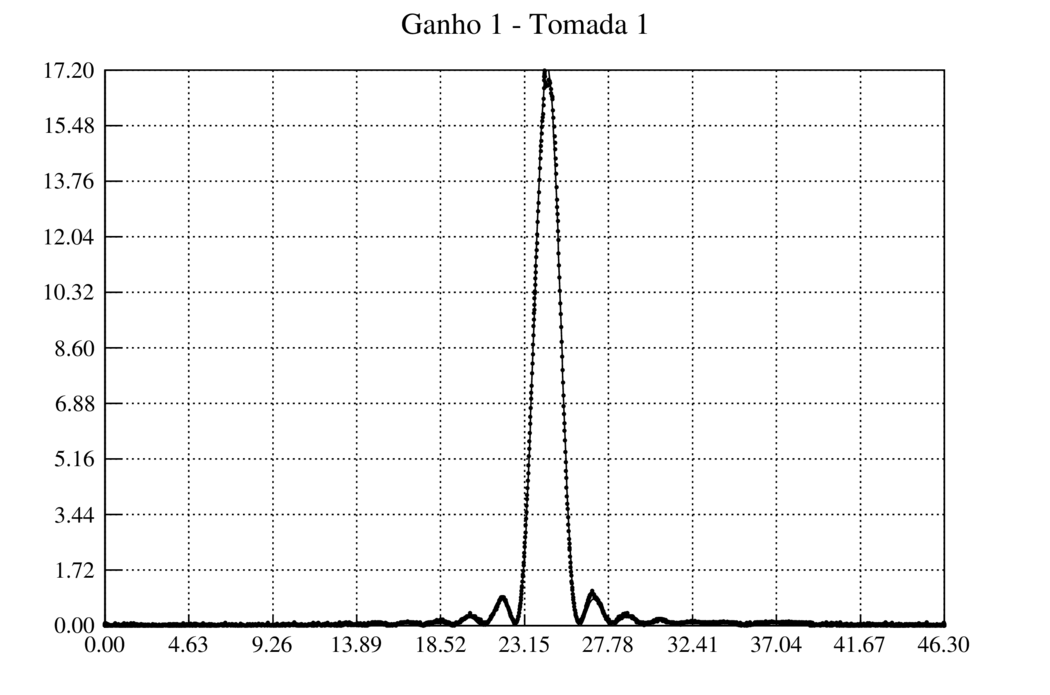
\includegraphics[scale=0.4]{g1.png}
   \caption{Dados ajustados do experimento}
   \label{meu_rotulo}
  \end{figure}
  
\subsection{Criação de Tabelas}    
  
  \item Segue na Tabela \ref{tabela} algumas derivadas de funções:
  \begin{table}[!htb]
   \centering
    \begin{tabular}{|c||c|}
     \hline
     Função & Derivada \\ \hline
     $f(x) = x^n$ & $f'(x) = nx^{n-1}$ \\ \hline
     $f(x) = \log_a x$ & $f'(x) = \dfrac{1}{\ln a}$ \\ \hline
    \end{tabular}
    \caption{Tabela Básica de Derivadas}
    \label{tabela}
  \end{table}
  
\end{enumerate}


\end{document}